s\documentclass[12pt,oneside,a4paper,english]{article}
\usepackage[T1]{fontenc}
\usepackage[margin=2.25cm,headheight=26pt,includeheadfoot]{geometry}
\usepackage[english]{babel}
\usepackage{listings}
\usepackage{color}
\usepackage{titlesec}
\usepackage{titling}
\usepackage[framed, numbered]{matlab-prettifier}
\usepackage{changepage}
\usepackage{amsmath}
\usepackage{hyperref}
\usepackage{enumitem}
\usepackage{graphicx}
\usepackage{fancyhdr}
\usepackage{lastpage}
\usepackage{caption}
\usepackage{tocloft}
\usepackage{setspace}
\usepackage{multirow}
\usepackage{titling}
\usepackage{float}
\usepackage{comment}
\usepackage{booktabs}
\usepackage{indentfirst}
\usepackage{lscape}
\usepackage{booktabs,caption}
\usepackage[flushleft]{threeparttable}
\usepackage[english]{nomencl}
\usepackage{xcolor}
\usepackage{lipsum}
\usepackage[utf8]{inputenc}
\usepackage{array}
\usepackage{multirow}
\usepackage{ragged2e}
\usepackage{multicol}


% --- set footer and header ---
\pagestyle{fancy}
\fancyhf{}

\setlength{\parindent}{2em}
\title{CDIO - Del 3} % to reference as \title, dont use \maketitle
\makeatletter\let\Title\@title\makeatother



\lstset{language=Matlab,
style=Matlab-editor,
basicstyle=\normalsize\mlttfamily,
numbers=left,
numberstyle={\scriptsize\color{black}},			% size of the numbers
numbersep=0.5cm											
}

\newlist{steps}{enumerate}{1}
\setlist[steps, 1]{leftmargin=1.5cm,label = Step \arabic*:}
\renewcommand{\headrulewidth}{1pt}
\renewcommand{\footrulewidth}{1pt}

%\lhead{\Title}
\rhead{\nouppercase{\rightmark}}
\lhead{\Title}
\rfoot{
\includegraphics[height=1.25cm]{root/logo.pdf}} % right header logo
\setlength\headheight{16pt}
\setlength{\footskip}{50pt}
\lhead{\Title} %rightH title
\cfoot{\thepage}

% --- End of page settings ---

\begin{document}
\pagenumbering{roman} 
\begin{titlepage}
\begin{center}
\begin{multicols}{2}
\addtolength{\topmargin}{-.5cm}

%\textsc{ Danmarks Tekniske Universitet}\\[1.5cm]

\includegraphics[width=0.45\textwidth]{root/dtu.png}~\\
\vspace{.5cm}


62532\\ Versionsstyring og testmetoder \\
\vspace{.2cm}
62531\\ Udviklingsmetoder til IT-systemer \\
\vspace{.2cm}
02312\\ Indledende programmering \\
\end{multicols}{}
\vspace{.5cm}

% Title
\hrule
\vspace{.5cm}
{ \huge \bfseries  CDIO - Del 3} % title of the report
\vspace{.5cm}

\hrule
\vspace{1cm}

\textsc{\textbf{Authors}}\\

\begin{center}

% add your name here
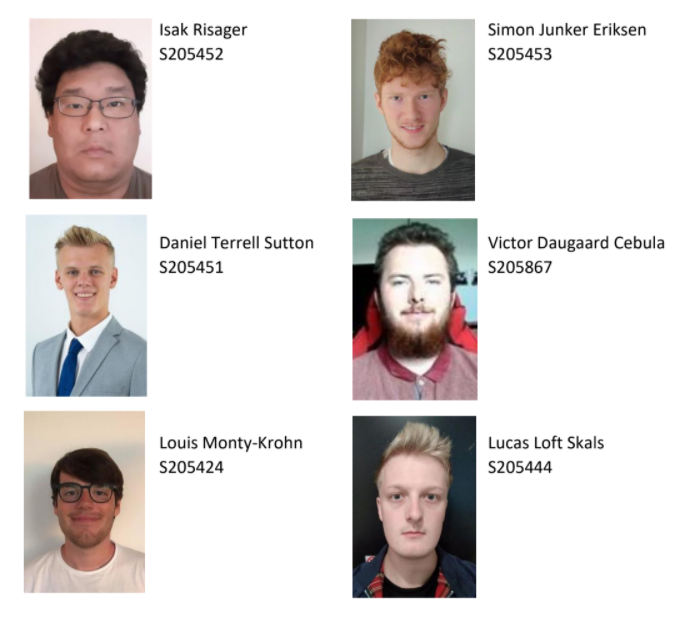
\includegraphics[width=0.9\textwidth]{Report/ProfilePictures/Forsidebilleder_vert.png}\\

\end{center}

27-11-2020

\vspace{0.1cm}

Gruppe 24
\end{center}
\end{titlepage}

\newpage
\begin{flushleft} % sætter tekststarten i venstre marginside.

\begin{center}
    \vspace{0.9cm}
    \textbf{Abstract}
\end{center}
\doublespacing

In the present project, we developed a Monopoly Junior game for Windows OS users. The project followed a Unified Process style of workflow including the following two phases: elaboration and construction. The analyses for the project included a requirements specification, actor and use-case analyses and a domain analysis. The designs for the project included a system-sequence, sequence and design class analyses. The implementation resulted in a playable Monopoly Junior game with some bugs which included entering a player's age with out-of-bounds parameters. For tests, JUnit tests were conducted for each relevant software class along with a user test for the entire program. 

\addlinespace
\url{https://github.com/louismonty/24_del3}
\end{flushleft}
\thispagestyle{fancy}

\newpage
\doublespacing
%\addcontentsline{toc}{section}{Table of Contents}
\renewcommand{\baselinestretch}{1}\normalsize
\tableofcontents
\renewcommand{\baselinestretch}{1}\normalsize
%\singlespacing
\thispagestyle{fancy} % force page style



\newpage
\section{Timeregnskab}
\centering
\begin{tabular}{ |c|c|c|c|c|c|c|  }
 \hline
 \multicolumn{7}{|c|}{Timeregnskab (timer)} \\
 \hline
 Aktivitet & Lucas & Victor & Simon & Louis & Daniel & Isak\\
 \hline
 
 
 Programmering      & 0 & 0 & 0 & 19 & 18 & 18 \\
 
 Møder              & 7 & 4 & 4 & 8 & 8 & 8 \\
 
 Rapportskrivning   & 26 & 4.5 & 1 & 1& 0 & 2 \\
 
 \hline
 
 I alt              & 33 & 8.5 & 5 & 28 & 26 & 28 \\
 
 
 \hline
\end{tabular}
\thispagestyle{fancy}
\pagenumbering{arabic} 
\fancyfoot[C]{Page \thepage\ of \pageref{endOfDoc}}


\newpage
\section{Kravspecifikation}
\input{Report/sources/2_Kravspecifikation}
\thispagestyle{fancy}

\newpage
\section{Analyse}
\input{Report/sources/3_Analysis}
\thispagestyle{fancy}

\newpage
\section{Design}
\input{Report/sources/4_Design}
\thispagestyle{fancy}




\end{document}

